\section{Experimentación y Resultados}

Mediante la presente sección se busca demostrar que tan eficaz y eficiente puede resultar la red neuronal para responder a las diversas situaciones presentadas durante el ajedrez cuántico.

Por ser un proyecto dedicado a lo que son entornos de juego, dentro de sus simulaciones propias la red neuronal creerá que está tomando decisiones correctas, mientra que en ambientes reales esto puede cambiar considerablemente dependiendo de como se le presenten nuevas situaciones a la red neuronal de las cuales tendrá que aprender para poder mejorar. Terminando con estas aclaraciones, se procederá a ver lo referido a todo lo referido a los experimentos realizados.

\subsection{Setup Experimental}
\subsubsection{Datos usados}

Para el presente trabajo, hay que recalcar algunos detalles. En este caso específico, los datos usados para los experimentos detallados a continuación han tenido que ser generados por computadora, sometiendo al entorno de juego a experimentos usando tres tipos de casos con el fin de obtener datos suficientes y necesarios para entrenar la red neuronal que será la encargada de jugar al ajedrez cuántico. Con esta finalidad, se han definido dos tipos de jugadores: \textbf{Random Player} (es un jugador que toma decisiones completamente aleatorias, no hace un análisis altamente profundo y representa a los jugadores muy novatos en el ajedrez, permitiendo una generación de datos altamente veloz) y \textbf{Montecarlo Player} (representa a jugadores más experimentados haciendo un análisis profundo de las situaciones de juego; cabe resaltar que, debido al análisis que realizará, el procesado de las jugadas será mucho más lento que en el tipo de jugador previamente mencionado). Finalmente, las formas en las cuales se han conseguido los datos han sido las siguientes:

\begin{enumerate}
    \item Random Player vs Random Player: 
    \item Ramdom Player vs Montecarlo Player:
    \item Montecarlo Player vs Montecarlo Player: 
\end{enumerate}

Con la finalidad de optimizar la ejecución y la obtención de datos, se ha tenido que realizar estas ejecuciones de manera independiente, en diversas líneas de ejecución. Además, debido al tamaño de las ejecuciones, después de haber terminado una simulación, se han tenido que eliminar los datos en caché de las simulaciones previas a medida que avanzan, para poder realizar las simulaciones con mayor eficacia.

Referido a esto, se usaron dos formas de obtener los datos. La primera requirió el propio trabajo de Google Colaboratory para generar datos; sin embargo, las limitaciones propias del sistema impiden una generación amplia, que era lo requerido para el trabajo presentado. Por lo tanto, se recurrió al uso de instancias de Amazon Web Services (AWS) para optimizar y llevar a cabo esta tarea con mayor rapidez, aprovechando que el sistema de Amazon tiene mayor potencia para generar datos y mantenerse ejecutando cuando los jugadores Montecarlo simulan partidas entre sí, ya que requieren un alto consumo de memoria que recientes actualizaciones de Google Colaboratory han restringido a los usuarios.

Por último, cabe resaltar que los datos obtenidos se han almacenado en un archivo CSV, lo que permitirá cargar los datos en la red neuronal.

\subsubsection{Métricas de evaluación}

\paragraph{Perdida (Loss)}
La función de pérdida que será utilizada es \textbf{"categorical crossentropy"}. Esta misma función se le asignó a cada cabezal; no obstante, como convergen todos en la capa anterior, debido a que comparten todas las capas menos la de salida, se mantendrá el análisis de pérdida tomando las pérdidas como un todo y no como predicciones independientes.

No se asignarán pesos a cada pérdida, ya que todos los componentes del vector tienen el mismo valor, y se deberán analizar como una única predicción. No se tomará un promedio de pérdidas, porque si sucede un error en algún cabezal, es necesario que esta afecte rotundamente a la pérdida total, cosa que, si se promediaba, su error no sería tan influyente para el entrenamiento, y requerimos su magnitud absoluta. Es por esto que la función final de pérdida será:

\[ L_{\text{total}} = \sum_{i=1}^{n} -\frac{1}{m} \left( \sum_{j=1}^{m} \sum_{k=1}^{c} y_{jk} \log(\hat{y}_{jk}) \right) \]

donde: 
\begin{align*} 
n &= \text{Número de salidas} \\ 
m &= \text{Número de muestras} \\ 
c &= \text{Número posible de resultados} \\ y_{jk} &= \text{Resultado real} \\ \hat{y}_{jk} &= \text{Resultado predicho} \end{align*}

\paragraph{Error Absoluto Medio(MAE)}
Esta métrica será utilizada para determinar el rendimiento de la red neuronal; lo que se realizó fue asignar esta función a cada uno de los cabezales. De esta manera, como se tendrá un MAE por cabezal a la hora de evaluar el modelo, realizaremos un promedio para conocer el desempeño general de la red neuronal empleada. Se hizo selección de esta métrica porque mide qué tan cerca están las predicciones de los valores reales, sin requerir una coincidencia exacta. Justamente no se pretende que se tenga algo muy cercano a lo real, porque debido a la cantidad de posibles resultados resulta improbable; por ello, cuanto menor sea el MAE, implica que se tienen muy buenos resultados.

\paragraph{Algoritmos de optimización}

Ya que se requiere hacer un análisis de grandes cantidades de jugadas, se requiere tener algoritmos que permitan hallas la mejor posible (optimizando el resultado). Como parte de la investigación y experimentación, se comparará el proceso de mejora del fitness de cada uno de los algoritmos (Greedy Search y SBMA). Esto se realizará guardando el mejor fitness, que se representa por la función presentada en la sección de metodología, por cada iteración de mejora que realice cada uno de los optimizadores. Luego con estos datos se realizará una gráfica para realizar las evaluaciones de sus desempeños. Ambos funcionarán bajo la misma cantidad de capas, y la misma función de fitness, para que ambos estén bajo la misma métrica, finalmente esta se calculará mediante la metodología de Train-Test.

\subsubsection{Configuración experimental}

Para la generación del dataset, se hará uso de la instancia en AWS mencionada previamente en la metodología, además de sesiones en Google Colaboratory, utilizando la CPU.

Por otro lado, para la optimización de hiperparámetros se utilizará, de igual manera, el último software mencionado. Sin embargo, para evitar problemas con la memoria RAM, debido a la cantidad de posibles soluciones y modelos generados, se utilizó una v2-8 TPU, ya que está proporcionaba 334.56 GiB de memoria RAM.

Una vez conseguidos los hipermetamorfosis optimizados, se procederá a comparar, mediante validación cruzada, el desempeño de la red utilizando SGD y Adam como optimizadores. Dado que la cantidad de modelos es menor, se hará uso de la sesión de tipo T4 GPU para otorgar velocidad en el entrenamiento.

Conseguido el mejor optimizado, y manteniendo la misma sesión, se realizará el entrenamiento final del modelo ya seleccionado.

\subsubsection{Escenarios probados}
\paragraph{Escenario 1: Redes aleatorias}
\textbf{Descripción:} Inicialmente se tienen una cantidad aleatoria de neuronas por capa, esta cantidad de capas se define inicialmente con 6; y los límites de neuronas por capas es de [0; 1024].\\
\textbf{Objetivo:} Inicializar todo para comenzar el ajuste.\\
\paragraph{Escenario 2: Red ajustada}
\textbf{Descripción}: Una vez se haya culminado con la optimización de hiper parámetros ya se tiene una red con un MAE adecuado, y un peso igualmente regulado.\\
\textbf{Parámetros}:
\begin{enumerate}
    \item Neuronas por capa: [ 561; 9; 176; 293; 1008; 95]
    \item Fitness: 0.8765378294944639        
\end{enumerate}
\textbf{Objetivo}: Tener ya una configuración para la red definida.\\

\paragraph{Escenario 3: Optimizador seleccionado}
\textbf{Descripción}: Con la red ya elegida se procedió a seleccionar un optimizador entre SGD y Adam basándose en los resultados de una cross validación.\\\\
\textbf{Parámetros}:
\begin{enumerate}
    \item Optimizador Seleccionado: SGD
    \item 1-MAE: 90.854       
\end{enumerate}
\textbf{Objetivo}: Tener un optimizador para ya conseguir un modelo completo para el entrenamiento.\\

\paragraph{Escenario 4: Entrenamiento y resultados}
\textbf{Descripción}: Una vez que la red ya está preparada, se genera el modelo final y se entrena. Para luego ser evaluado\\
\textbf{Parámetros}: MAE--> 8.899\%\\
\textbf{Objetivo}: Entrenar el modelo y analizar la minimización del MAE.\\

\subsubsection{Estrategia de validación}

Para validar en los algoritmos de optimización se utilizó \textit{Train-Test}; por otro lado, para la evaluación de los optimizadores de la \textit{MLP}, se utilizó \textit{Cross Validation} (en este caso, para hallar el resultado total se utilizó un promedio). En la división de datos, esta fue de un 25\% para pruebas, y 75\% para entrenamiento.

\subsection{Experimentación}
\subsubsection{Resultados:}
\paragraph{Resultados SBMA vs Greedy Search}
Con el fin de evaluar el desarrollo del experimento por iteración entre cada uno de los algoritmos de optimización.

\begin{center}
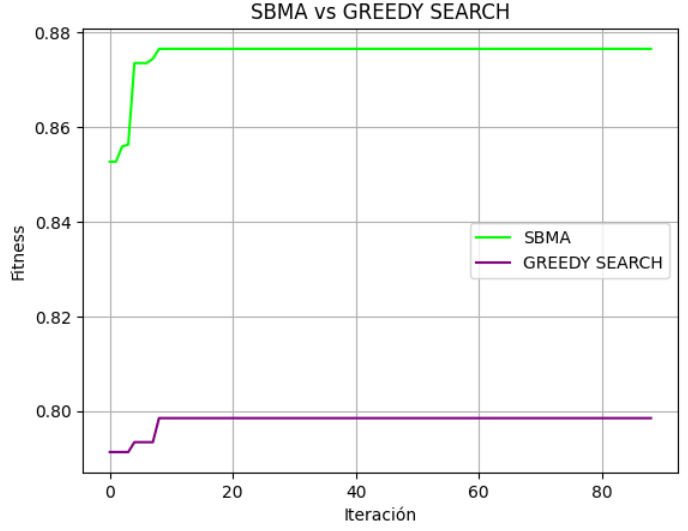
\includegraphics[scale=0.3]{Imagenes/Imagen.png}    
\end{center}

\paragraph{Resultados SGD vs Adam}
\subparagraph{Adam: }
Los resultados son de: 1-MAE: mean=90.654 std=0.148, Cantidad de Folds = 5

\begin{center}
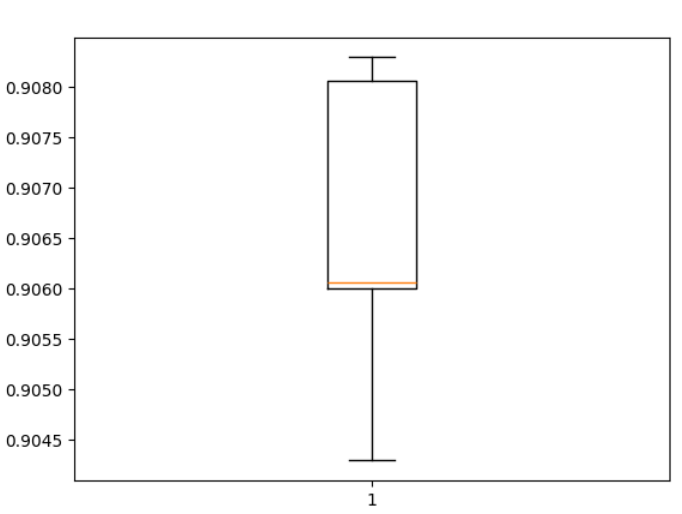
\includegraphics[scale=0.3]{Imagenes/uuh.png}
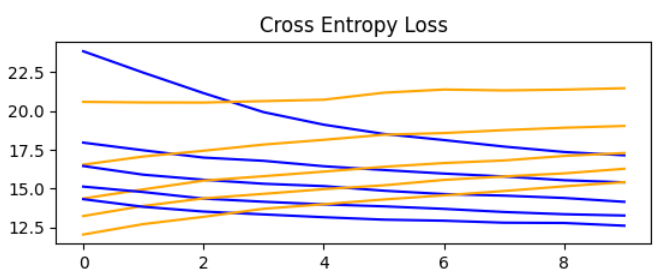
\includegraphics[scale=0.3]{Imagenes/image2.png}    
\end{center}

Se puede observar según el boxplot la media de 1-MAE es de 90.654\%, además según las curvas de cross entropy loss, al usar Adam, si bien no hay overfitting, hay mucha diferencia entre las pérdidas al momento de realizar los test y entrenamientos.

\textbf{SGD: } Los resultados son de: 1-MAE: mean=90.854 std=0.714, Cantidad de Folds = 5.

\begin{center}
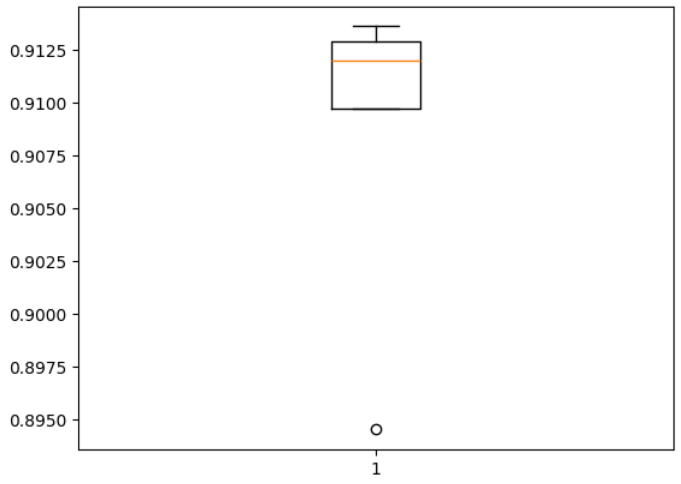
\includegraphics[scale=0.3]{Imagenes/image6.png}
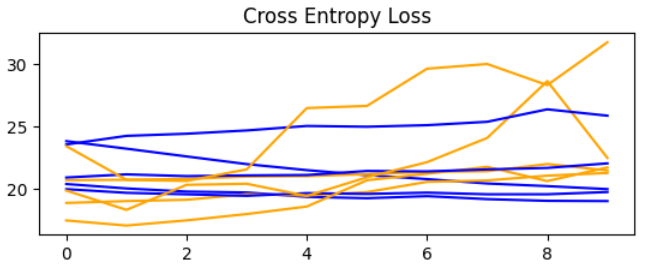
\includegraphics[scale=0.3]{Imagenes/7gh.png}    
\end{center}

Según la mediana del boxplot, se tiene un 91\% de 1-MAE; por lo que se tienen mejores resultados con este optimizado. Sumado a esto, las curvas si bien hay ocasiones en las que se disparan las de pruebas, las demás si mantienen una mejor relación con sus contrapartes de entrenamiento
\subsubsection{Resultados finales}

\begin{center}
\begin{tabular}{c c c}
    \parbox[c]{2cm}{\centering Movimiento:\\ 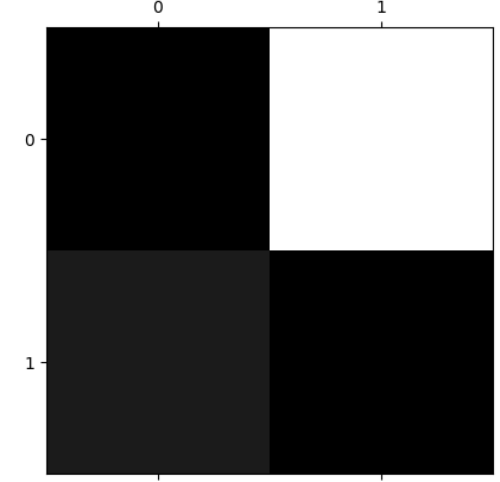
\includegraphics[width=2cm, height=2cm]{Imagenes/ghfg.png}} &
    \parbox[c]{2cm}{\centering Inicio 1:\\ 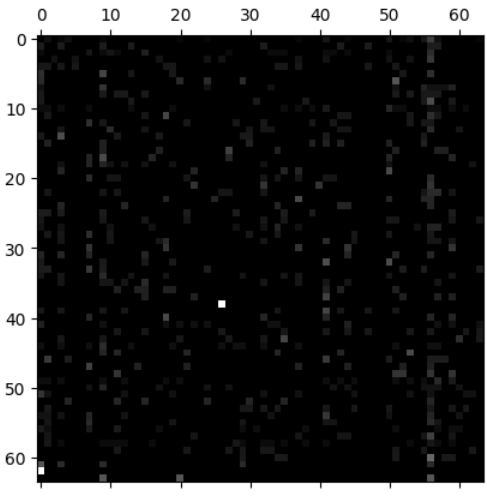
\includegraphics[width=2cm, height=2cm]{Imagenes/uuui.png}} &
    \parbox[c]{2cm}{\centering Inicio 2:\\ 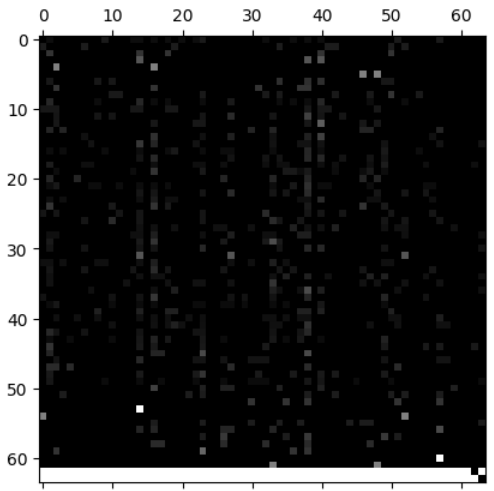
\includegraphics[width=2cm, height=2cm]{Imagenes/hg.png}} \\

    \parbox[c]{2cm}{\centering Fin 1:\\ 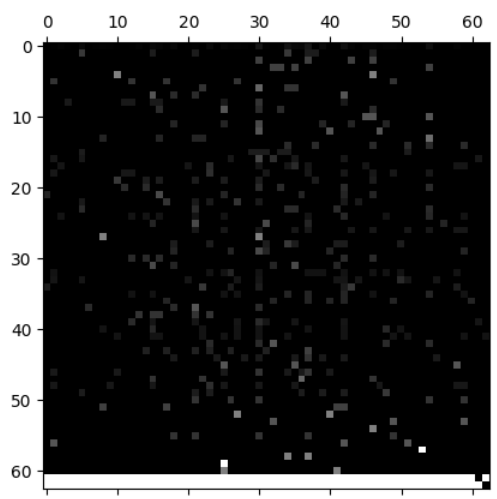
\includegraphics[width=2cm, height=2cm]{Imagenes/599.png}} &
    \parbox[c]{2cm}{\centering Fin 2:\\ 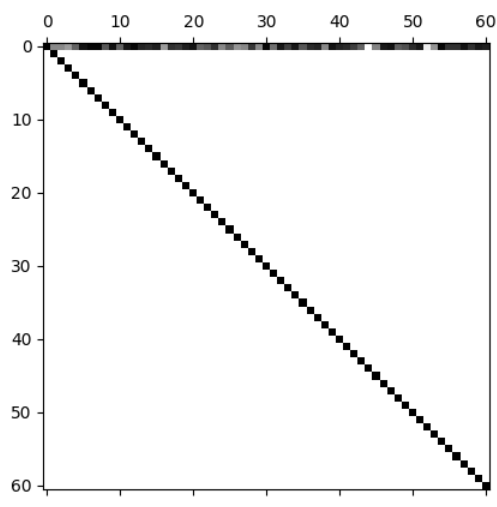
\includegraphics[width=2cm, height=2cm]{Imagenes/54o.png}} &
    \parbox[c]{2cm}{\centering Coronación:\\ 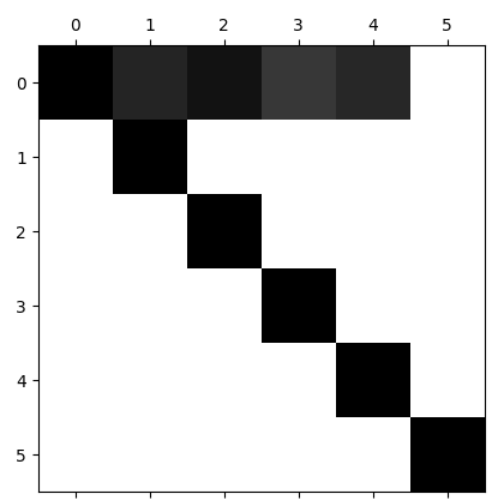
\includegraphics[width=2cm, height=2cm]{Imagenes/vvvvv.png}} \\
\end{tabular}
\end{center}